\documentclass[review,5p,times,twocolumn]{elsarticle}

\usepackage{algorithm,algorithmic}
\usepackage{amssymb}
\setcounter{tocdepth}{3}
\usepackage{graphicx}
\usepackage{amsmath}
\usepackage[printonlyused]{acronym}
\usepackage{tabularx}

\newcommand\markerlessfootnote[1]{%
  \begingroup
  \renewcommand\thefootnote{}\footnote{#1}%
  \addtocounter{footnote}{-1}%
  \endgroup
}

\newenvironment{Algorithm}[1]{\begin{minipage}{1\textwidth}\centering\begin{minipage}{#1}\begin{algorithm}[H]}
{\end{algorithm}\vspace{0.1cm}\end{minipage}\end{minipage}}

\newcommand{\INDSTATE}[1][1]{\STATE\hspace{#1\algorithmicindent}}
\newcommand{\indItem}{\setlength\itemindent{25pt}\item}

\newacro{DSDI}{Display Shape Dependence Issue}

\journal{Displays}

% Document starts
\begin{document}

\begin{frontmatter}

%% Title, authors and addresses

%% use the tnoteref command within \title for footnotes;
%% use the tnotetext command for the associated footnote;
%% use the fnref command within \author or \address for footnotes;
%% use the fntext command for the associated footnote;
%% use the corref command within \author for corresponding author footnotes;
%% use the cortext command for the associated footnote;
%% use the ead command for the email address,
%% and the form \ead[url] for the home page:
%%
%% \title{Title\tnoteref{label1}}
%% \tnotetext[label1]{}
%% \author{Name\corref{cor1}\fnref{label2}}
%% \ead{email address}
%% \ead[url]{home page}
%% \fntext[label2]{}
%% \cortext[cor1]{}
%% \address{Address\fnref{label3}}
%% \fntext[label3]{}

\title{Repositioning Visual Content To Fit Different Tabletop\\Display Shapes}

%% use optional labels to link authors explicitly to addresses:
%% \author[label1,label2]{<author name>}
%% \address[label1]{<address>}
%% \address[label2]{<address>}

\author[durham]{James McNaughton\corref{correspondent}}
\ead{j.a.mcnaughton@durham.ac.uk}
\author[cardiff]{Tom Crick}
\ead{tcrick@cardiffmet.ac.uk}
\author[newcastleEng]{Shamus P. Smith}
\ead{Shamus.Smith@newcastle.edu.au}
\author[newcastleCha]{Elizabeth Burd}
\ead{Liz.Burd@newcastle.edu.au}

\cortext[correspondent]{Corresponding author. Phone: +44 (0) 191 33 44312}

\address[durham]{Technology Enhanced Learning Special Interest Group, School of Education, Durham University, South Road, Durham, DH1 3LE, UK}
\address[cardiff]{Department of Computing \& Information Systems, Cardiff Metropolitan University, Cardiff, CF5 2YB, UK}
\address[newcastleEng]{ES248, Callaghan, University Drive, Callaghan NSW 2308, Australia}
\address[newcastleCha]{CH320A, The Chancellery, Callaghan, University Drive, Callaghan NSW 2308, Australia}


\begin{abstract}
Advances in technology are transforming the capabilities of system interfaces.
Previously, the majority of systems have utilised rectangular displays.
This may soon change.
At present, software is usually designed assuming its use with a display of a specific shape.
There may soon be the need for tabletop-orientated systems to be capable of handling a wide range of potential display shapes.
The design of software for use on a range of differently shaped tabletop displays is considered in this work.
A generic technique which can be used to minimise the influence of the issues of using different display shapes was developed.
Observations on the technique explore how it can be used to adapt the layout of tabletop software to different display shapes.
\end{abstract}


\begin{keyword}
Visual content management \sep irregular displays \sep screen design
\end{keyword}


\end{frontmatter}

%-------------------------------------------------------------------------
\section{Introduction}
\label{sec:intro}

Most tabletop software systems that provide visual feedback to a user are normally designed to do so with a particular display shape.
The most common of these display shapes is the rectangle.
However, adapting displays to different shapes has always been possible through covering regions of a display~\cite{Dietz2004}.
This, in addition to new technologies such as circular liquid crystal displays~\cite{Boyd2007,Finney2009}, allows for different display shapes to be used in tabletop systems. 
Developers need to consider how to make their software flexible enough to adapt to not only displays of varying sizes and aspect ratios, but also to displays of varying shape.

The work discussed in this paper explores a technique that would allow developers to adapt tabletop software to different display shapes.
The remainder of this paper is as follows. 
Section~\ref{sec:related} outlines the current development and drive for non-traditional display shapes with tabletop systems. 
The issues arising from the use of different display shapes on a system are outlined in Section~\ref{sec:problem}.
A technique to minimise the influence of the identified issues is proposed in Section~\ref{sec:solution}.
The implementation of the technique into a software framework is discussed in Section~\ref{sec:study}.
Section~\ref{sec:observations} discusses the implications that arise from the technique use.
Future developments and our conclusions are presented in Section~\ref{sec:conclusion}.

%-------------------------------------------------------------------------
\section{Background}
\label{sec:related}

Traditional displays used in computer systems are mostly rectangular.
However, there is an increasing number of non-rectangular displays becoming available.
One such instance of a non-rectangular display is Toshiba's circular thin film transistor liquid crystal display~\cite{Boyd2007}.
This display is employed in vehicles to show typical dashboard information.
The display is made to look similar to a typical dial on a car dashboard.
This requires the display to be circular.
The Motorola Aura~\cite{Finney2009} is a phone that showcases another example of a non-rectangular display and in this case is another circular screen.

A non-rectangular display is utilised in the PyMT (Python Multi-touch)~\cite{Hansen2009} project.
A circular display is made by projecting the system's output onto a circular surface.
The \lq Puddle of Life\rq\ application is designed to tailor its visual output to this circular display shape.
This means that the software is constrained by the specifications of the hardware.
This is also true for software built for circular dashboard~\cite{Boyd2007} and phone~\cite{Finney2009} displays.
As a result, such software could not be used easily with other display shapes.
Therefore, applications used with these circular displays would not be suitable for use with typical rectangular displays.
The trend is for custom interface solutions, such as tabletop systems, on non-rectangular display shapes.

The DiamondSpin framework~\cite{Shen2004} offers support for circular tabletop multi-touch displays.
Instances of a circular display used by the framework are achieved through either projecting the system's visual output onto a circular surface or occluding sections of the output.
DiamondSpin~\cite{Shen2004} supports these displays through several applications which are designed specifically for use on a circular tabletop interface.
The framework provides several features to support applications intended for circular interfaces, such as the ability to orientate items towards the nearest edge of the display.
Some of the example applications for the DiamondSpin framework~\cite{Shen2004} can be used with both rectangular and circular interfaces.
Using the framework's features the applications are able to appropriately arrange the layout of content to the display shape used.
However, this adaptive ability is limited to two display shapes, rectangular and circular.

The circular dashboard liquid crystal display~\cite{Boyd2007} is a typical example of a technology designed with the intention of supporting ubiquitous computing~\cite{Weiser1999}.
It can be argued that an era of ubiquitous computing is beginning, where more systems will be designed to naturally fit into their surroundings~\cite{Greenfield2006}.
For computer systems to be ubiquitous they are required to be designed around typical user environments.
This differs from having user environments tailored around systems as has previously been the case.
The implication of this is that many previous standard elements of typical computing systems will need to be reconsidered, for example the shape of a system's interface.

Work that discusses the possible effects of displays with non-rectangular display shapes~\cite{Vernier2002} highlights the benefits it may offer.
These benefits include potential improvements to collaboration around the display between users.
Vernier et al.~\cite{Vernier2002} propose a circular tabletop interface which will allow each user to have an equal share of the display.
Though focused on a circular tabletop displays, they highlight the effect that a different display shape could have on the use of an interface.
Benefits noted in the work include the improved management of users' personal space.
One of the strengths of tabletop systems are their ubiquitous nature~\cite{Smith2012}.
The ability for a tabletop system to manage different display shapes enhances this strength allowing the interfaces to better fit its environment.

It is evident that the visual contents of systems will need to accommodate the use of different display shapes.
An obvious way to achieve this is to define specific layouts in software's visual content for each potential display shape it may be used with.
This is the approach used with the software systems discussed in this section thus far~\cite{Hansen2009,Shen2004}.
However, for software which may have a wide range of potential interface shapes this would require a significant amount of time.
A potential method to reduce this time is to use a tool which can adapt the layout of visual contents to different platforms, such as GUMMY~\cite{Meskens2008}.
This tool can take an existing layout, defined by a software developer, and can quickly adapt it to the parameters of a specific platform, including the restrictions of the display.
For example, the spacing of a predefined layout may be reduced by the tool when the target platform is known to use a small display.
By implementing a method which allows the tool to dynamically adapt a layout of content items to different display shapes, software developers could produce multiple layouts for a piece of software to use with different display shapes relatively quickly.

As opposed to using predefined layouts for each potential display shape, software could be designed to use a single layout which is adapted to fit different display shapes automatically.
For example, SUPPLE~\cite{Gajos2004} is a system which can automatically adapt the layout of contents to fit the parameters of the display.
Content is arranged by the system to fit various display sizes and resolutions.
SUPPLE~\cite{Gajos2004} also has the ability to adapt its visual contents based on the type of input used by the system.
However, the system assumes that despite the changes in an interface's size, resolution, input type and colour support, it will always be rectangular.
Changes to layout adapting systems, like SUPPLE~\cite{Gajos2004}, will be needed to allow them to adapt their layouts to non-rectangular displays.

There exists initial research into software capable of adapting its visual contents to different display shapes.
Waldner et al. \cite{Waldner2011} discuss work carried out concerning the development of a system which allows windows to be adapted to make use of unusual display shapes.
The unusual display shapes discussed by Waldner et al. consist of a series of overlapping projections which form the system's output.
These overlapping projections will not always form a rectangular shape.
Therefore, it is important for the software used not to be dependent on a rectangular visual output.
The technique works by finding the best location for new windows.
An importance value is used for each pixel of the output and the magnitude of this value is used to assess its suitability to displaying a new window.
The higher the value is, the less suitable the pixel is.
Pixels outside the output's shape are given a maximal importance value.
This means that no window can be placed anywhere which will result in it occupying these pixels.
This prevents content windows being placed where they may be partially occluded due to some of their regions existing outside the display area.
This is beneficial as no visual content is obscured.

The technique of Waldner et al. \cite{Waldner2011} appears to be beneficial for use with windows which have no layout defined between each other.
The technique could be employed in other systems to manage the placement of visual content items when used with different display shapes.
However, for visual content which may have a significant locational relationship this technique could be considered unsuitable.
The order in which windows are created will influence where the technique positions them.
Therefore, the technique currently has no method to accommodate for any locational relationships which are intended to exist between windows.
If two visual content items are intended to be in close proximity to each other, there is no guarantee that the technique will position them together.
As the positioning of content items can imply their functional relationships to the user~\cite{Constantine1999}, the loss of these intended locational relationships could be undesirable for some systems.

The potential benefits~\cite{Greenfield2006,Vernier2002} and growing supporting technologies~\cite{Boyd2007,Finney2009} of non-rectangular displays indicate that there is an increasing demand for systems to support them.
Specifically there is a growing demand for these different display shapes in tabletop systems~\cite{Hansen2009,Shen2004}.
For tools which are used to design the layout of software~\cite{Meskens2008} or systems which dynamically update the layout of visual content items~\cite{Gajos2004}, a method of adapting visual content layouts to different tabletop display shapes will be needed.
%-------------------------------------------------------------------------
\section{Identifying Display Shape Dependence Issues}
\label{sec:problem}

For developing a method of adapting visual content layouts to different display shapes, the effects of applying a new display shape to a system's visual output need to be considered.
Issues can occur when a display shape which differs from the shape of a display assumed by the software is used.
In this section we define six of these \acp{DSDI}.

\begin{quote}\emph{\textbf{Cropping \ac{DSDI}} Content items appear cropped as regions of them become positioned outside the display area.}\end{quote}

Cropping can have an effect of making the effected visual content items unfit for purpose.
This is because the visual information they convey is lost.
Users may also be unable to interact directly with cropped items.
The cropping of visual content items outside the display area was also noted by Waldner et al. \cite{Waldner2011}.
This influence could result in content becoming unfit for purpose which may result in software becoming unusable.
Therefore, methods of resolving this cropping would be required to make software capable of adapting to different display shapes.
Attempts made to resolve this cropping can result in secondary \acp{DSDI}.

 \begin{figure*}[t]
 \centering
   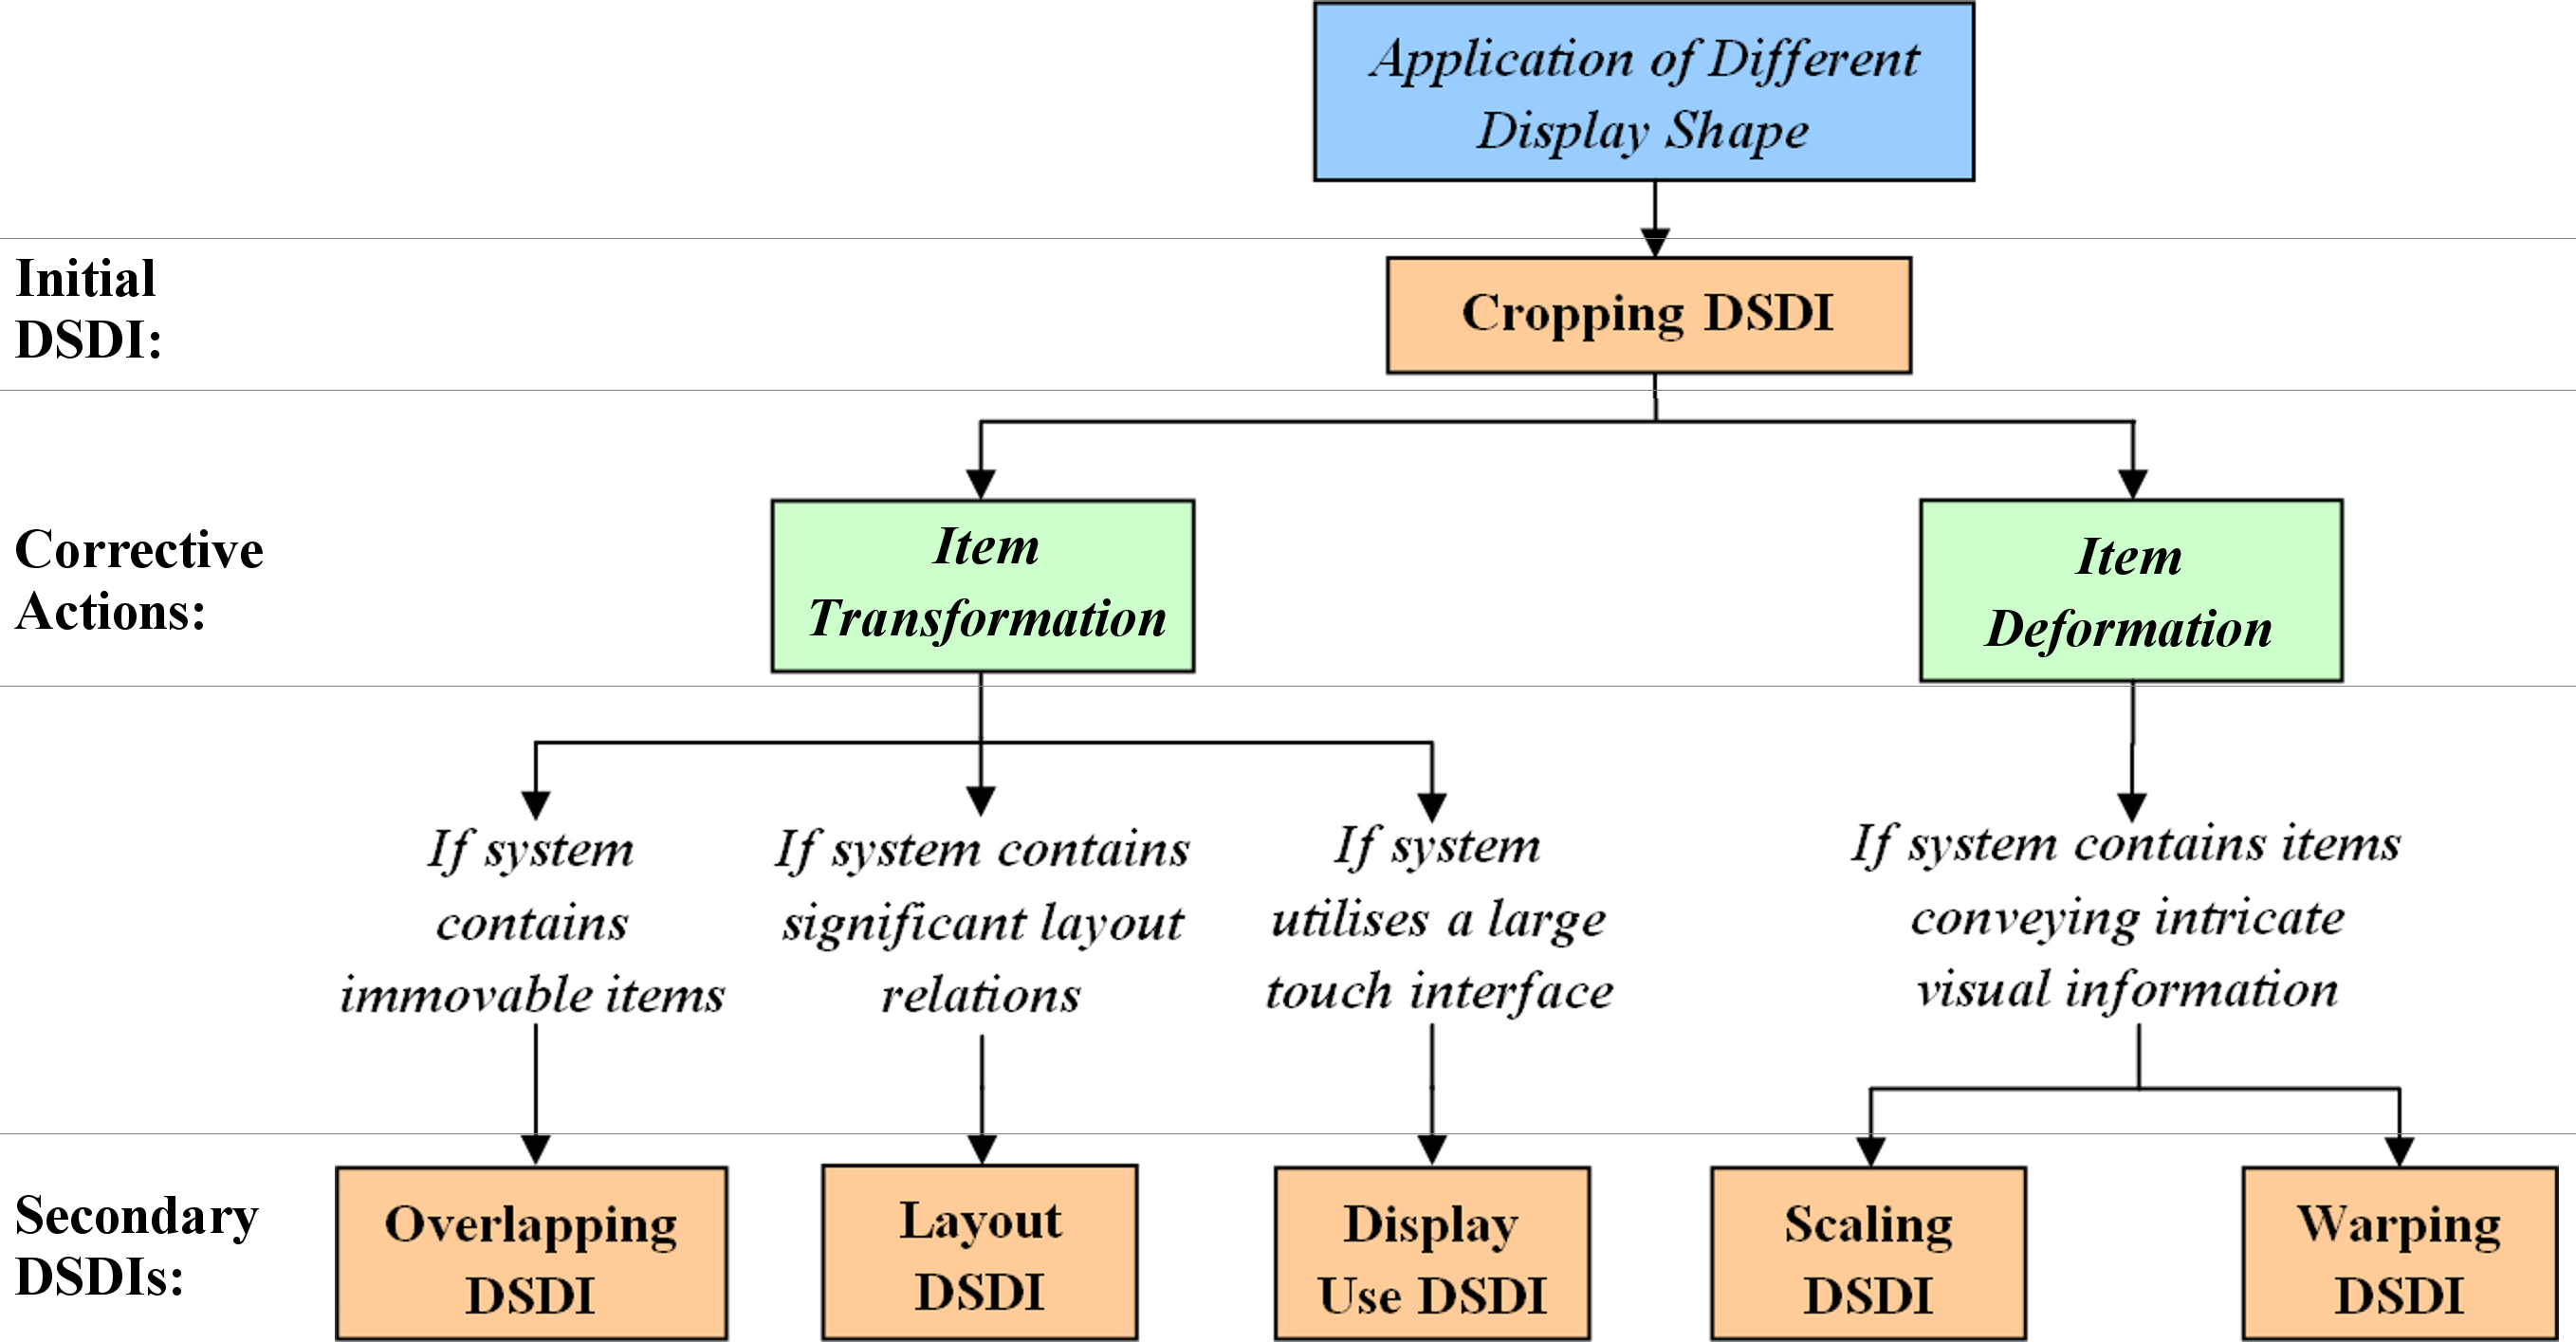
\includegraphics[width=1\textwidth]{figures/dsdi_flow.png}
   \caption{A flow chat mapping the causality of \acp{DSDI}.}
   \label{fig:dsdiFlow}
\end{figure*}

\begin{quote}\emph{\textbf{Overlapping \ac{DSDI}:} Occlusion from other visual content items.}\end{quote}

Attempts to resolve the Cropping \ac{DSDI} can result in further issues such as the movement of content items, which did not previously overlap, to locations where they cover each other.
However, this can result in content items, which previously did not overlap, covering each other.
This overlapping of content items can result in regions of the visual content item becoming obscured.
This has the same negative impact as the Cropping \ac{DSDI}.
Overlapping content items is not always an issue since the obscuring items could be moved by the user, but in systems where these items are immovable the occlusion would be irreparable.

\begin{quote}\emph{\textbf{Layout \ac{DSDI}:} The loss of layout relations between visual content items.}\end{quote}

The changing of content item positions could be an issue in applications where layout is important.
This is because the positioning of content items can imply their functional relationships to the user~\cite{Constantine1999}.
For example, controls in an application may be placed next to the items they influence.
If this layout relation is lost then it may become users what items the set of controls will influence. 
The loss of layout may not make content unfit for purpose but could be very undesirable for software where the layout is intended to aid the user.
However, loss of layout is not always considered an issue meaning this \ac{DSDI} will only apply to specific content, tasks or applications.

\begin{quote}\emph{\textbf{Scaling \ac{DSDI}:} The scaling of visual content items to an extreme.}\end{quote}

Scaling, when a content item is resized while maintain its aspect ratio, a visual element may be performed to avoid the cropping of content.
If this scaling is performed to an excessive magnitude, the visual information displayed by a content item may become incommunicable.
For example, if a content item displaying text is scaled down to an extreme value the characters it displays become too small and may appear illegible to users.

\begin{quote}\emph{\textbf{Warping \ac{DSDI}:} The warping of visual content items.}\end{quote}

Warping is where the contents of a system are stretched and/or squashed in a non-uniform manner~\cite{Milliron2002}.
This could be applied to the entire visual output of a system to make it fit a particular display shape.
However, this results in content items being stretched and squashed non-uniformly.
Even when the magnitude of this deformation is relatively small it can make any visual information a content item displays incommunicable to the user.
However, this \ac{DSDI} may not apply in all circumstances.
Some visual content items may display visual information which is communicable to the user no matter how extremely it is deformed.
For example, if a content item's visual information is its colour; if the item can be seen then it is successfully communicating its visual information to the user.

\begin{quote}\emph{\textbf{Display Use \ac{DSDI}:} Display regions unused by the layout of visual content items.}\end{quote}


As a result of attempting to resolve the initial cropping, visual content items can often be translated to the same regions of the display.
This can leave large areas of an interface unused.
While this may not make the software unfit for purpose it is not desirable for large tabletop interfaces.
This is due to the fact that on larger interfaces some regions of the display may be beyond a user's reach.
If the display uses direct touch interaction, then items in these regions become isolated from the user's influence.
There are solutions to this problem, such as users changing their positions around the interface or controls which can be used to indirectly manipulate out of reach items~\cite{Ryall2006a}.
However, if all the content items are constrained to a single region of the display beyond a user's reach, the need to repeatedly use these solutions is undesirable.
Changing positions to access remote content may not be possible in some environments due to the placement of the interface.
Multi-touch interfaces may have several users positioned around them.
Users interacting simultaneously with a single interface often have a tendency to establish territories~\cite{scott2004}.
A user wishing to move with these types of interfaces may disrupt others interacting with the system.
Solutions involving the remote control of out of reach content items result in users manipulating content items through a proxy~\cite{Smith11}.
This means that their interaction would no longer be direct.
This can be undesirable because it counteracts the benefits of direct touch interaction~\cite{Schoning2008}.
Ensuring content items are capable of being spread out across the interface when possible reduces the likelihood that all the items will be placed beyond the reach of the users.

For a tabletop software system to be capable of dynamically adapting its visual content to different display shapes, the Cropping \ac{DSDI} needs to be resolved in such a manner that will minimise the influence of any of the potential secondary \acp{DSDI}.
Figure~\ref{fig:dsdiFlow} maps the causality of the \acp{DSDI} and notes the circumstances in which they may have undesirable consequences on a system's visual content.
With this list of \acp{DSDI}, a technique to adapt software to different display shapes in such a way that reduces the possibility of software becoming unusable due to these issues has been developed.

%-------------------------------------------------------------------------
\section{Minimising Display Shape Dependence Issues}
\label{sec:solution}

A technique was developed that would resolve the Cropping \ac{DSDI} and would minimise the effect of any secondary \acp{DSDI}.
This technique is a method of adapting visual content items dynamically to different display shapes.
The technique comprises of two stages.
The first stage of the technique is built on the concept of taking the original visual output of the software and transforming it to fit within the borders of a new display shape.
This stage is referred to as {\em Virtual Projection}.
The second stage of the technique uses the difference between the shape of virtual projection and the display shape to ensure that the layout can, if needed, utilise all regions of the display.
This stage is referred to as {\em Position Pulling}.


\subsection{Virtual Projection}
\label{subsec:virtualprojection}

\begin{figure}[h]
 \centering
   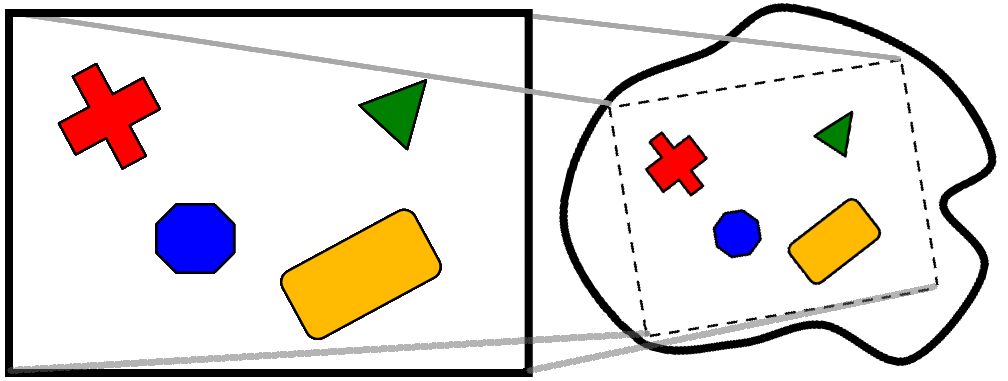
\includegraphics[width=0.45\textwidth]{figures/virtual_rectangle.png}
   \caption{An example of the Virtual Projection stage.}
   \label{fig:virtualRectangle}
\end{figure}

For the first stage of the technique, the original shape of the software environment's visual output is treated as a single item.
This item, referred to as the virtual projection, is translated, rotated and scaled so that it fits within the display shape being used.
The transformations applied to the virtual projection are applied to any visual content items displayed in the software's original layout.

\begin{algorithm}[h]
\caption{Applying virtual projection transformation.}
\label{algo:virtualProjection}
\begin{algorithmic}
\STATE \textbf{virtualProjection}(item, $\overrightarrow{translation}$, rotation, scale)
\INDSTATE[2]$item.rotateBy(rotation)$
\INDSTATE[2]$item.translateBy(\overrightarrow{translation})$
\INDSTATE[2]$item.scaleBy(scale)$
\end{algorithmic}
\end{algorithm}

Algorithm~\ref{algo:virtualProjection} shows how the virtual project transformation is applied to visual content items.
The translation, scaling and rotation fed into the algorithm relate to the virtual projection.
These can obtained be either being recorded when the maximal rectangle is found or calculated on the fly by comparing it to the maximal rectangle of a typical rectangular display.
The algorithm is applied to each visual content item with the transformations being relative to the item's initial absolute positioning.

This stage of the technique has the effect of keeping the visual content items aligned with the virtual projection.
This ensures that visual contents will not incur occlusion from lying outside the borders of the new display shape.
This is because the content items will all be contained within the virtual environment which fits inside the display.
Figure~\ref{fig:virtualRectangle} demonstrates how the virtual projection and its contents are transformed together to fit a new display shape.

As the original visual output of most current software is likely to be rectangular, the virtual projection for most systems can assumed to be a rectangle.
Finding the largest rectangle which can be placed within the display is required for this technique to utilise as much of the display as possible.
The concept of finding the largest rectangle inside a shape is a known as the \lq largest empty rectangle problem\rq\ or the \lq maximal rectangle problem\rq .
There are several existing solutions to finding the maximal rectangle which can be utilised~\cite{Aggarwal1987,Naamad1984}.

Methods also exist for finding the largest of any specific polygon in the display shape~\cite{Toussaint1983}. 
This allows for the adaptation of any software environment which may not have originally been rectangular.
Therefore the technique can be used to adapt software originally designed for any specific display shape to other display shapes.

As all the content items are translated, rotated and scaled by the same values their layout relations are preserved preventing the Overlapping \ac{DSDI}.
As no warping deformations are used in this technique there can be no occurrence of the Warping \ac{DSDI}.

There is the potential occurrence of the Scaling \ac{DSDI}.
If the virtual projection is significantly smaller than the initial layout's environment, then the contained content items will be scaled to an extreme value.
It is possible that the content items may be scaled to an extent that they become unfit for purpose.
To counter this the virtual projection technique adheres to scaling limits.
For systems where content items cannot be scaled to extremes, its content items should only be scaled to a predetermined limit.
This may result in sections of the content items becoming occluded from overlapping each other or from the display edge because they cannot be made small enough.
Without scale limits, the Cropping and Overlapping \acp{DSDI} are guaranteed not to occur but the Scaling \ac{DSDI} remains a risk.
With scale limits the potential \acp{DSDI} are reversed.
When utilising this technique, developers must decide on \ac{DSDI} trade-offs in their software.

This stage of the technique is similar to previously presented methods of dynamically adapting content to different displays which entails constricting the placement of content to a specific region of the displays used~\cite{Cotting2006,Raskar2003}.
This region is recreated for every display shape using the same dimensions, ensuring the contained content is kept relative to the region in layout, scale and orientation.

This stage of the technique does have the potential to minimise the effects of most of the \acp{DSDI}.
However, this stage of the technique does not counter the occurrence of the Display Use \ac{DSDI} since only a single region of the display, the virtual projection, is used.

\subsection{Position Pulling}
\label{subsec:positionpulling} 

\begin{figure}[h] 
 \centering
   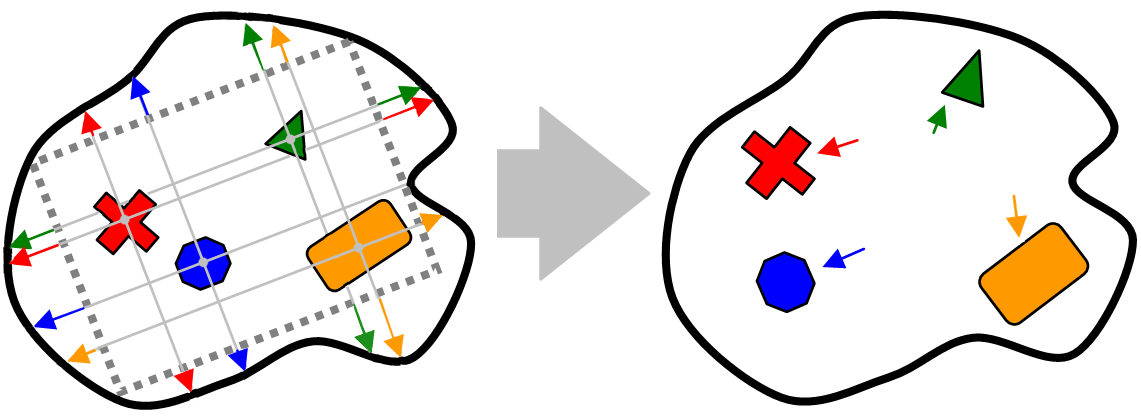
\includegraphics[width=0.45\textwidth]{figures/virtual_rectangle_pull_example.png}
   \caption{An example of the Position Pulling stage.}
   \label{fig:pullLayout}
\end{figure}

For the second stage of the technique, the gaps between the virtual projection and the display edges are utilised.
The objective of this stage is to move content items into areas of the display which are left unused by the virtual projection.
The edges of the virtual projection exert a \lq pulling force\rq\ on content items.
The magnitude of this force is determined by the size of gaps between the display border and the virtual projection edges.
The magnitudes of these \lq pulling forces\rq\ are also influenced by a content item's proximity to the edge instigating the force.
Content Items are pulled from their centroids to keep calculations simple.
This means the shapes and sizes of the items moved are ignored.

The position pulling stage has the resulting effect of pulling content items into unused regions of the display (see
Figure~\ref{fig:pullLayout}).
Items positioned near large gaps between the virtual projection and the display borders are pulled into these areas.
The left hand side of Figure~\ref{fig:pullLayout} shows the \lq pulling forces\rq\ which result from the gaps between the virtual projection area edges adjacent to the content items.
Figure~\ref{fig:pullLayout}'s right hand side shows the translation of the content items resulting from the combined influence of the \lq pulling forces\rq .

\begin{figure}[h] 
 \centering
   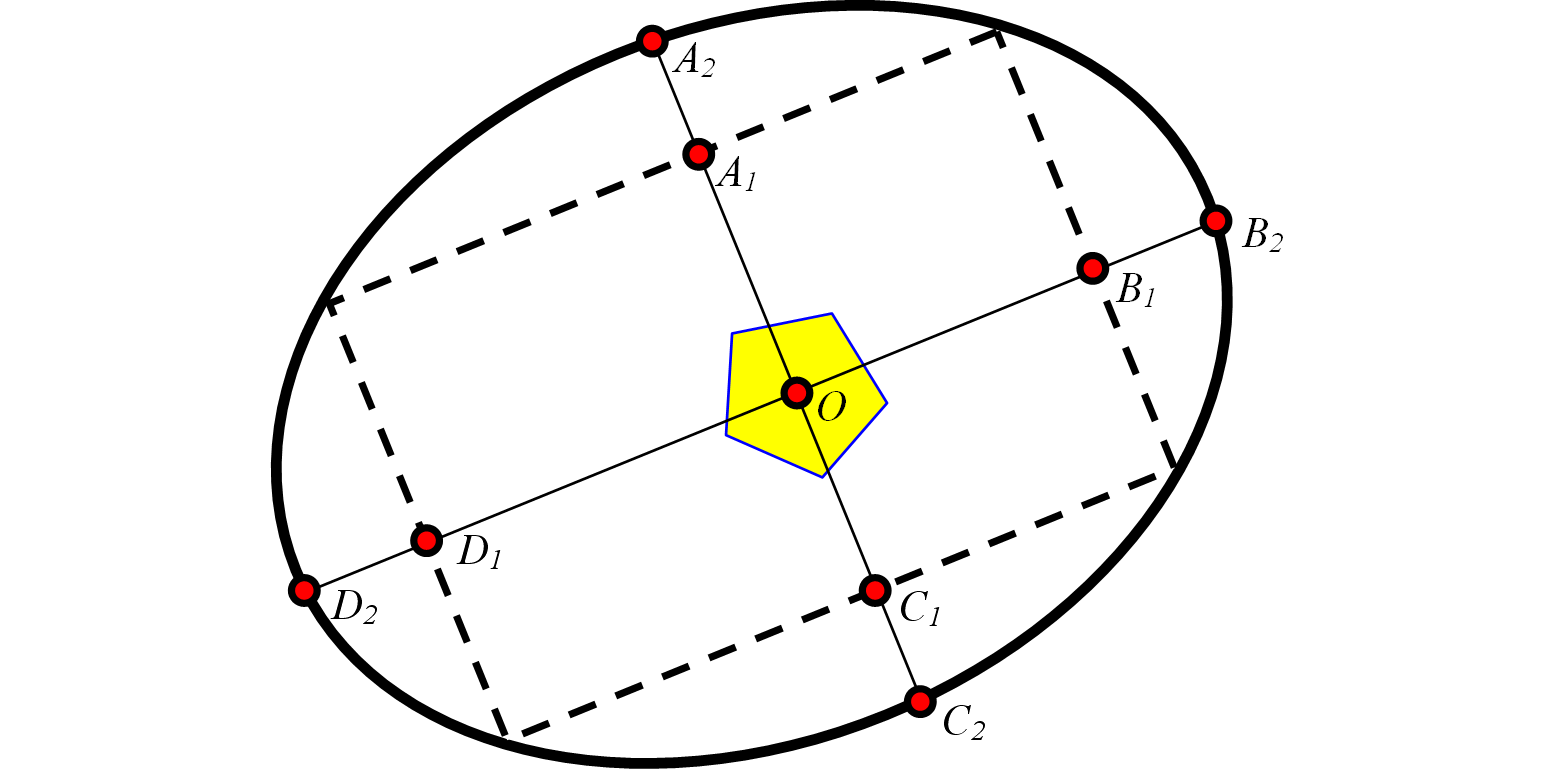
\includegraphics[width=0.45\textwidth]{figures/virtual_rectangle_pull_example_detailed.png}
   \caption{Detailed view of the information used in Position Pulling.}
   \label{fig:pullLayoutExp}
\end{figure}

\begin{algorithm}[h]
\caption{Calculating the \lq pulling force\rq vectors.}
\label{algo:pullLayoutOne}
\begin{algorithmic}
\STATE \textbf{getPullVectors}($O,\ A_{1},\ A_{2},\ B_{1},\ B_{2},\ C_{1},\ C_{2},\ D_{1},\ D_{2}$)
\INDSTATE[2]$\overrightarrow{LEFT}\hspace{0.5cm} \leftarrow \hspace{0.25cm}(\overrightarrow{D_{1}D_{2}}\ *\ ( |\overrightarrow{OD_{1}}|\  /\ |\overrightarrow{B_{1}D_{1}}| )$
\INDSTATE[2]$\overrightarrow{RIGHT}\hspace{0.25cm} \leftarrow \hspace{0.25cm}(\overrightarrow{B_{1}B_{2}}\ *\ ( |\overrightarrow{OB_{1}}|\  /\ |\overrightarrow{B_{1}D_{1}}| )$
\INDSTATE[2]$\overrightarrow{UP}\hspace{1cm} \leftarrow \hspace{0.25cm}(\overrightarrow{A_{1}A_{2}}\ *\ ( |\overrightarrow{OC_{1}}|\  /\ |\overrightarrow{A_{1}C_{1}}| )$
\INDSTATE[2]$\overrightarrow{DOWN}\hspace{0.3cm} \leftarrow \hspace{0.25cm}(\overrightarrow{C_{1}C_{2}}\ *\ ( |\overrightarrow{OA_{1}}|\  /\ |\overrightarrow{A_{1}C_{1}}| )$
\STATE \textit{return}\ $\overrightarrow{LEFT},\ \overrightarrow{RIGHT},\ \overrightarrow{UP},\ \overrightarrow{DOWN}$
\end{algorithmic}
\end{algorithm}

\begin{algorithm}[h!]
\caption{Applying the \lq pulling force\rq vectors.}
\label{algo:pullLayoutTwo}
\begin{algorithmic}
\STATE \textbf{applyPull}($item,\ \theta,\ \overrightarrow{LEFT},\ \overrightarrow{RIGHT},\ \overrightarrow{UP},\ \overrightarrow{DOWN}$)
\INDSTATE[2]$\overrightarrow{PULL} \leftarrow \overrightarrow{LEFT} + \overrightarrow{RIGHT} + \overrightarrow{UP} + \overrightarrow{DOWN}$
\INDSTATE[2]$\overrightarrow{PULL}.rotateBy(\theta)$
\INDSTATE[2]$item.translateBy(\overrightarrow{PULL})$
\STATE \textit{return}
\end{algorithmic}
\end{algorithm}

Algorithm~\ref{algo:pullLayoutOne} shows how each vector representing the individual \lq pulling force\rq\ is calculated and made proportional to the item's proximity to the corresponding edge.
Algorithm~\ref{algo:pullLayoutTwo} details how the resulting vector is attained from these values then applied where $\theta$ represents the orientation of the virtual projection.
The existing values used in Algorithm~\ref{algo:pullLayoutOne} and Algorithm~\ref{algo:pullLayoutTwo} correspond to those shown in Figure~\ref{fig:pullLayoutExp}.

This stage of the technique effectively deforms the layout of the content items by warping~\cite{Milliron2002} it to fit the display shape.
Though the layout is warped, the content items are not deformed in any way by this stage of the technique technique.
The deformation of the layout ensures that more of the display's real estate is utilised and that the layout is not constrained to a small region of the display.
This minimises the potential effects of the Display Use \ac{DSDI}.
The shape of the item does not influence the pull vectors, only the point it uses for translation.
Taking the shape into account would require significantly more processing and would only result in a marginally more accurate pull vector.

The \lq pulling forces\rq\ used in this stage of the technique assume the original environment of a piece of software is rectangular.
Assuming a rectangular environment can be considered acceptable due to the current prevalence of software intended for use with rectangular displays~\cite{VanDam2001}.
However, it is possible that in the future the technique may need to adapt software designed for non-rectangular displays to different shapes.
The virtual projection stage can easily adapt to this through using the maximal polygon opposed to the maximal rectangle.
For the position pulling stage to utilise content intended for a non-rectangular display, a vector representing the \lq pulling force\rq\ for every unique edge of the virtual projection would need to be created.
Vector addition between each of these vectors representing the \lq pulling forces\rq\ then creates a single vector which can be used to translate a content item.

After employing the two stages discussed, the resulting technique has the potential to minimise the \acp{DSDI} identified, when different display shapes are utilised by a system. 
While the technique does has the ability to counter any \ac{DSDI}, it does have the drawback of requiring trade-offs in its implementation between which \acp{DSDI} it minimises the consequences of.

%-------------------------------------------------------------------------
\section{Study}
\label{sec:study}

The technique discussed in Section~\ref{sec:solution} was implemented into the 2.1 version of the SynergyNet framework~\cite{McNaughton2017,AlAgha2010}, a multi-touch software framework intended for use with rectangular tabletop interfaces.
The framework functions by rendering a range of content items, such as images, text and video, which can then be manipulated by users.
SynergyNet is built in Java allowing it to be run across different operating systems and can accept a wide range of different multi-touch protocols such as TUIO~\cite{Kaltenbrunner2007}.
This makes the framework capable of being used in a wide range of systems with different displays.
The framework's ability to adapt to different systems makes it a suitable candidate for use with different display shapes.
Another reason for this choice in framework was due to its easily accessed library of supported open-source applications.
Since the applications are produced by a number of different developers for different purposes, there is a wide range of content items and layouts available.
Being implemented at the framework level allows any of the supported applications to potentially utilise different display shapes.

To utilise the technique the software needs to be informed of the dimensions of the display shape being used.
This is done through the creation of virtual counterparts to the display shapes utilised by the system.
These virtual counterparts are represented as vector files which are loaded into applications through the framework's configuration interface.
The approach of using virtual counterparts allows each display shape representation to store information on the positioning of their maximal rectangle, or polygon.
The maximal rectangle can be used by the virtual projection stage of the technique because all the SynergyNet applications are currently built using a rectangular environment.

The technique is implemented in such a way that it is always employed when an application attempts to transform a content item using absolute values.
This means that, in addition to the initial positioning of content, the technique is employed when an application needs to transform an item to a specific position.
For example, if a new item is to be added to the `centre' of the visual content the technique would be applied to ensure it appears in the middle of the maximal rectangle, even if the item is added sometime after the application's initialisation.
The technique does not need to be utilised for relative transformations, such as those used when adjusting an item's position, scale or rotation in response to a user gesture.

The SynergyNet framework was adapted to apply a range of borders which would allow the display to emulate different shapes.
These shapes were chosen after consultation with a furniture manufacturer who had experience with designing multi-touch tables.
The manufacturer was in a good position for making predictions concerning the likely design features of future multi-touch tabletops, including their display shapes.
The shapes chosen are shown in Figure~\ref{fig:study} and Figure~\ref{fig:gridApp} in Section~\ref{sec:observations}.

Some of these shapes were derived from common table shapes which could be used with tabletop interfaces, such as the semi-circle design.
This allows for users positioned around the display in various places to have an equal share of the interface which can be beneficial to collaboration.
The circle shape was also chosen for its ability to allow users to have equal shares of the display.
The intersecting circles shape was designed to make further use of multi-touch's facilitation of collaboration by providing focal points and areas to share content items in.
The larger circle of the display shape can be used for one activity such as displaying content items whereas the smaller circle could be used for another activity such as manipulating the items.
The triangle was chosen because of its regular nature, meaning that all its sides and corners are congruent \cite{coxeter_1969}.
The other shapes used were identified as likely to aid collaboration which is beneficial to multi-touch systems~\cite{higgins2011}.

\begin{figure*}[t!] 
	\centerline{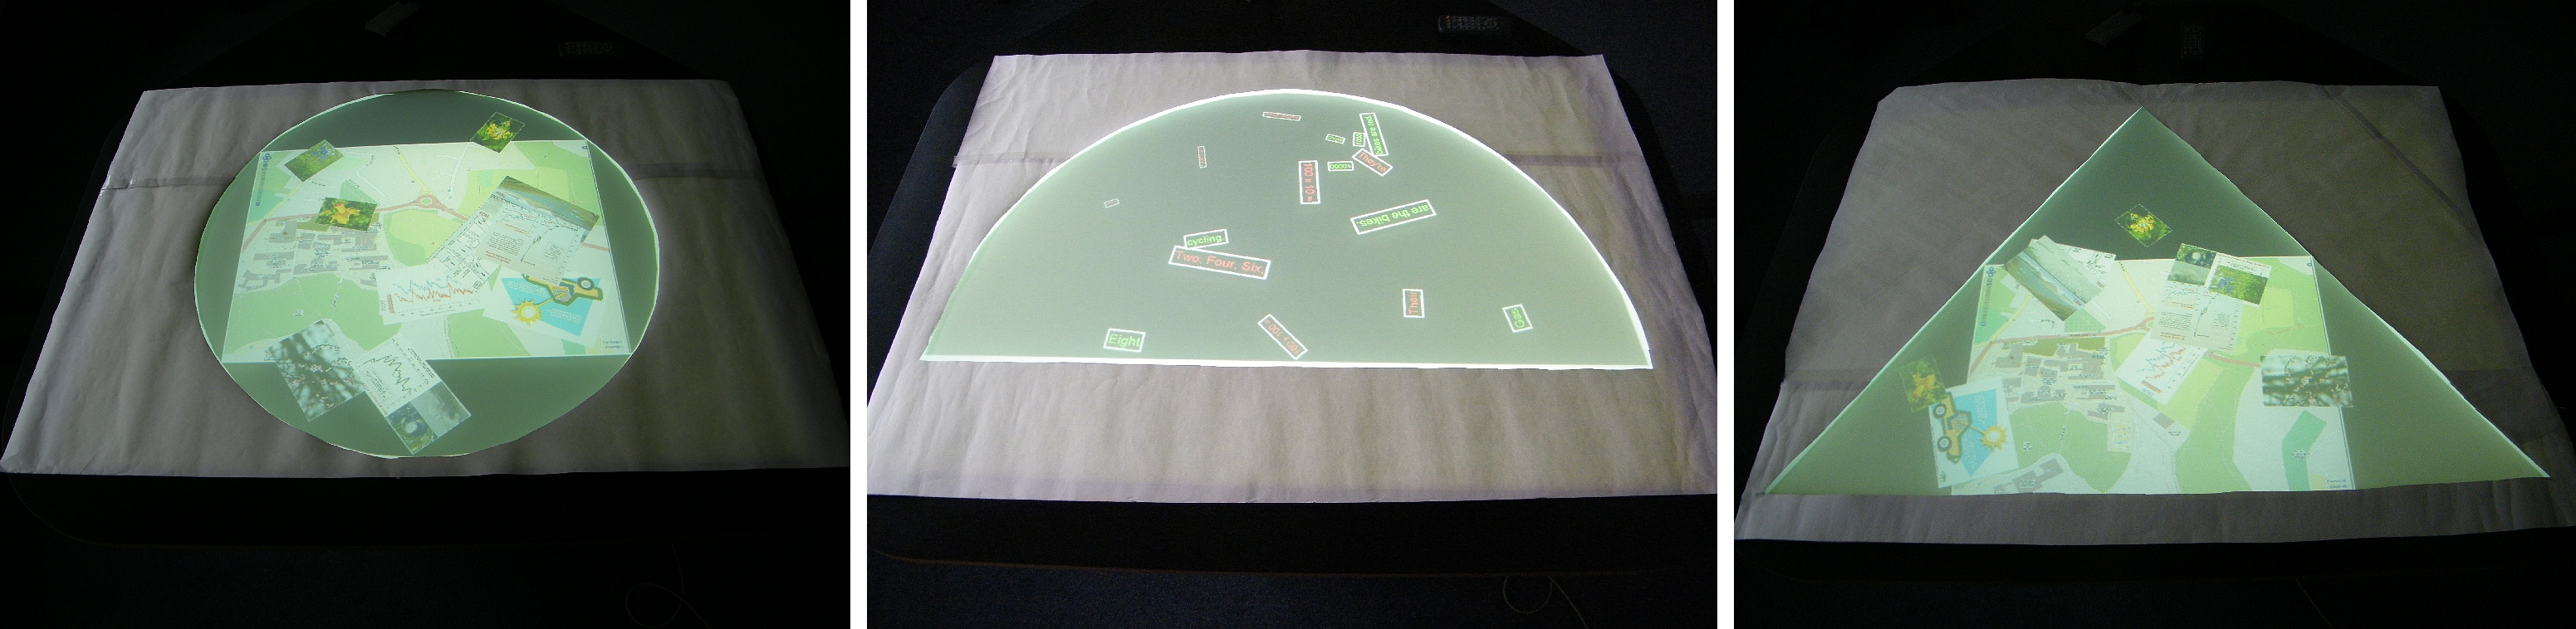
\includegraphics[width=1\textwidth]{figures/study.png}}
	\caption{Several applications in use with different display shapes during the study.}
	\label{fig:study}
\end{figure*}

With the technique implemented into the SynergyNet framework several applications were used in conjunction with a range of different display shapes.
The different display shapes were emulated by covering parts of the screen used.
Figure~\ref{fig:study} shows some of these applications in use with the various display shapes applied.
From the use of these applications observations were made on how the adaptation of their content to fit the new display shapes affected their initial usability.
Applications where the layout of content was significant in some way were focussed on.

%-------------------------------------------------------------------------
\section{Observations}
\label{sec:observations}

The majority of the applications were able to be utilised as normal with the \acp{DSDI} totally resolved.
Many of these involved randomly positioned content to which there was little or no significance to their layout.
However, two applications reliant on their visual contents highlighted a number of complexities to applying the technique.
These were the Grid and Simple Map applications.

\begin{figure*}[t!] 
	\centerline{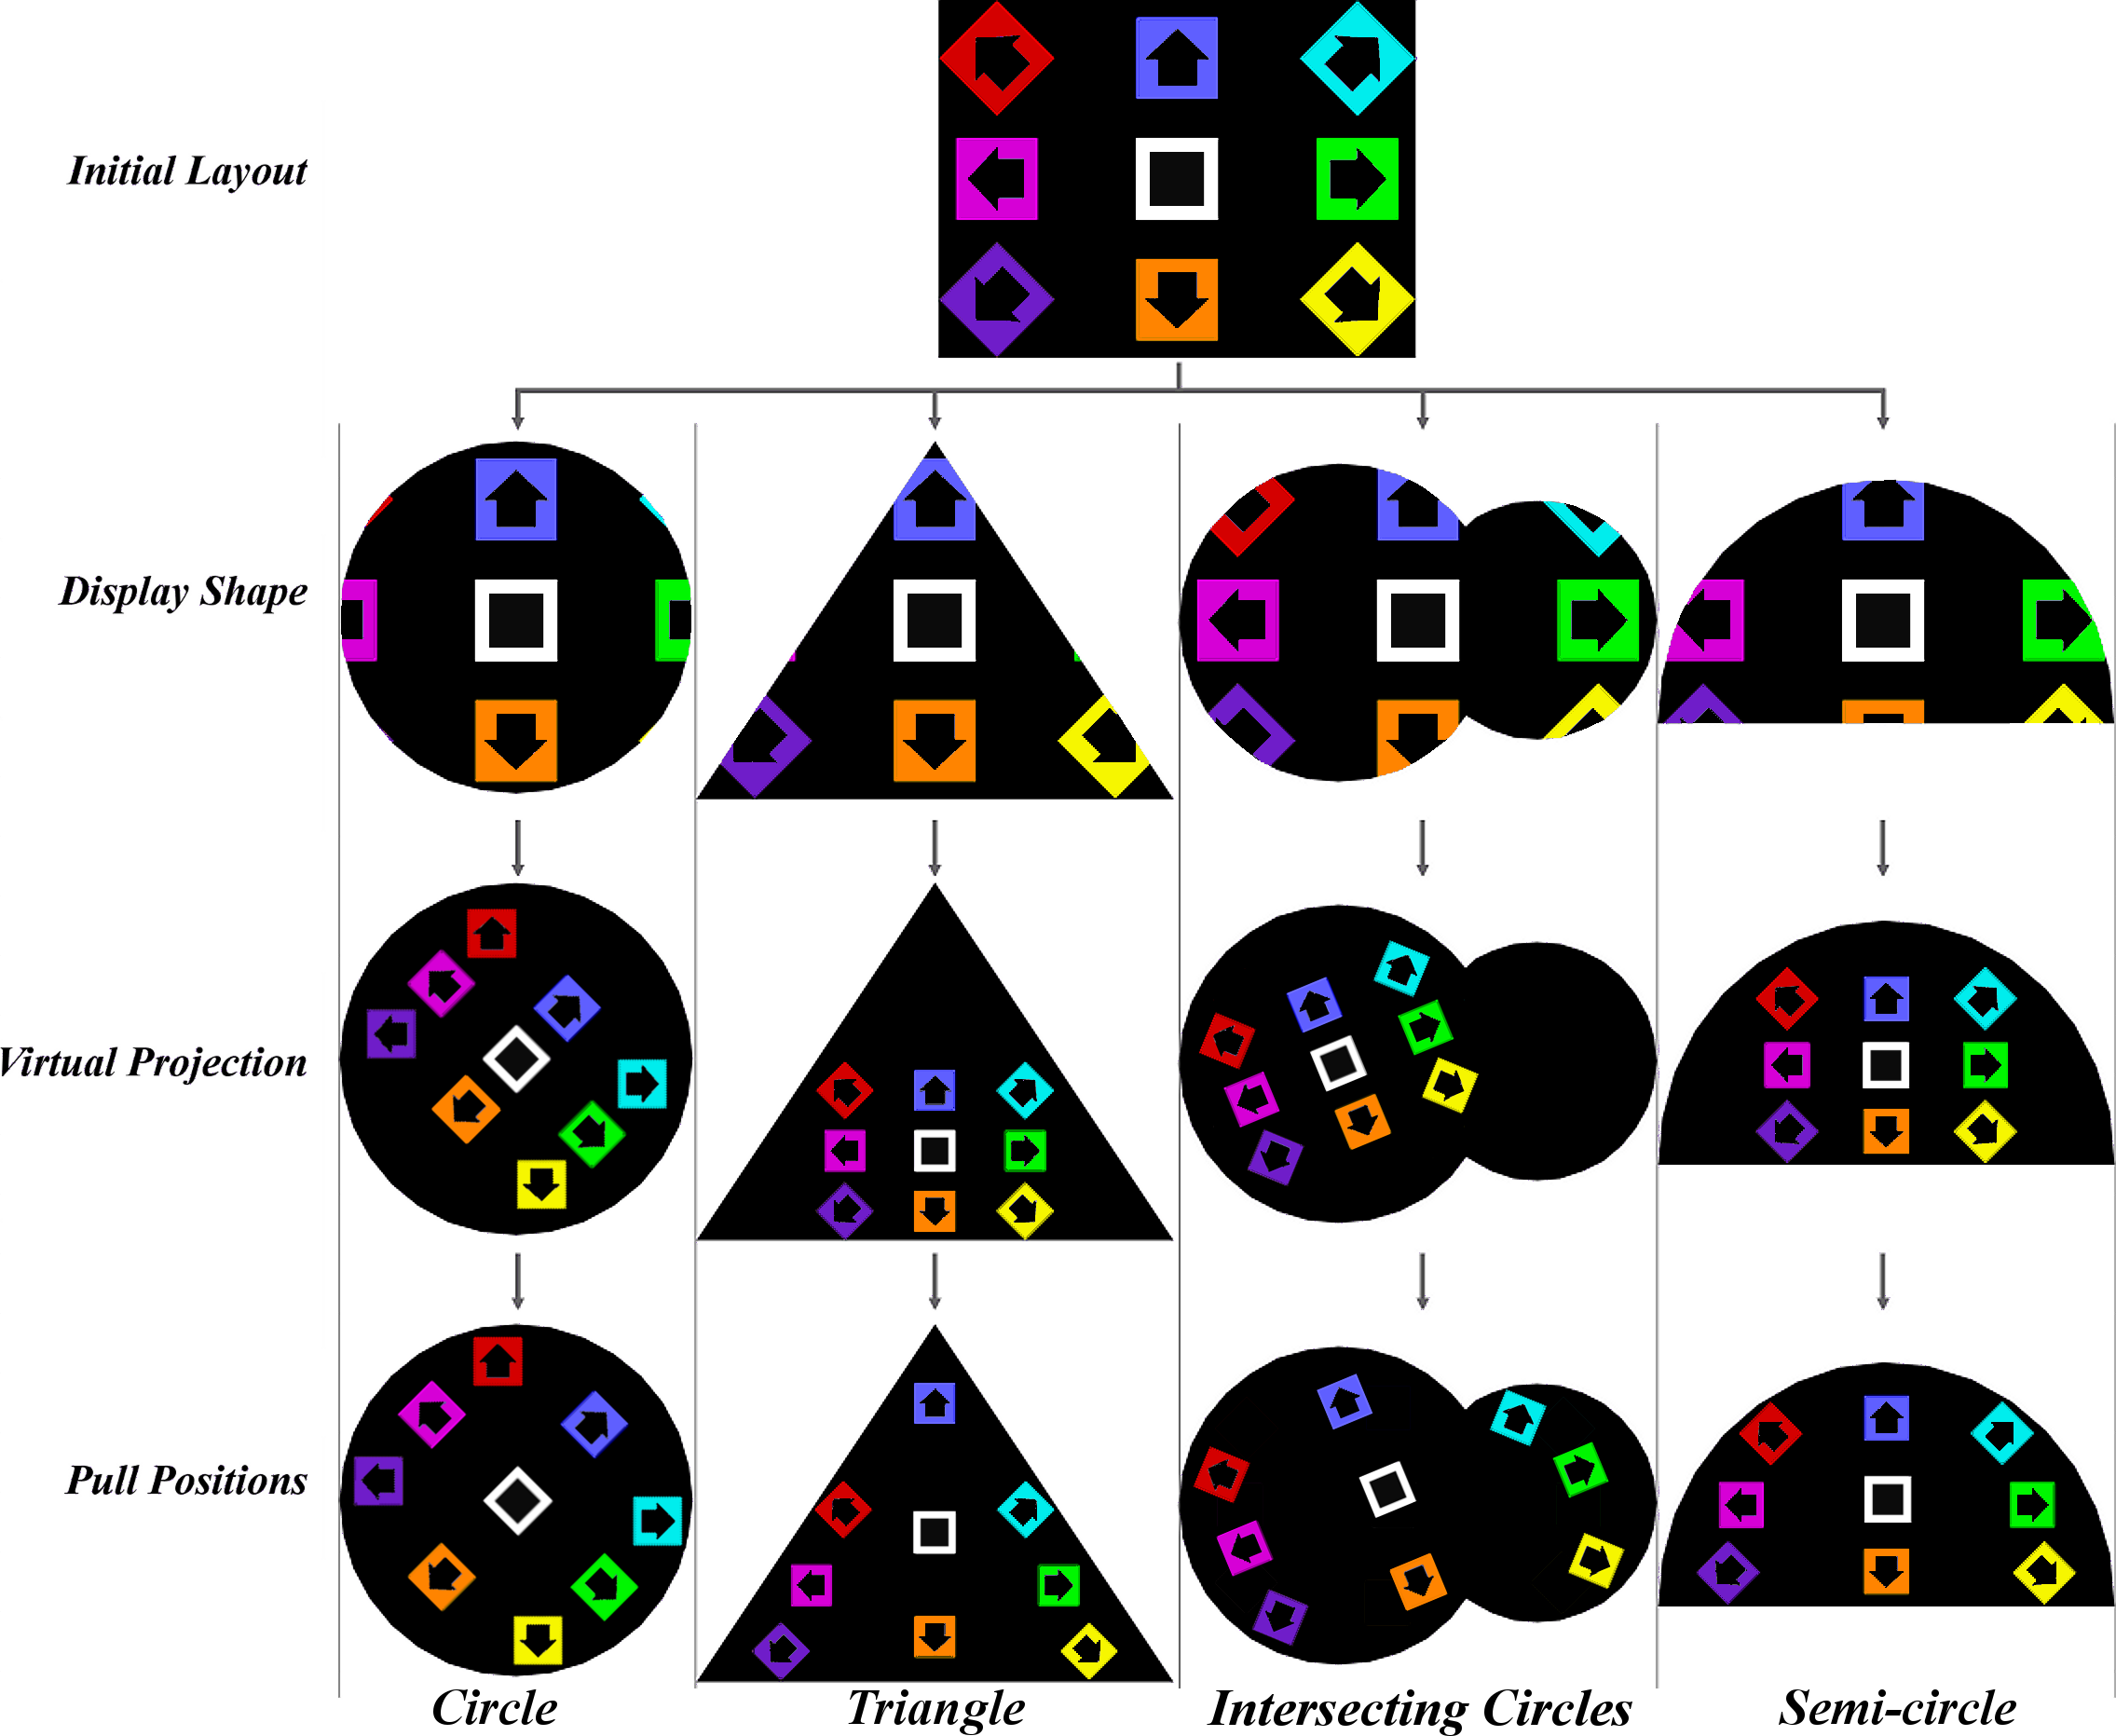
\includegraphics[width=1\textwidth]{figures/grid_app.png}}
	\caption{Influence of the implemented technique on SynergyNet's Grid application.}
	\label{fig:gridApp}
\end{figure*}

Figure~\ref{fig:gridApp} shows the Grid application which consists of nine items arranged in a grid so that the arrows, displayed by the items, point away from the centre of the display.  
As can be seen in Figure~\ref{fig:gridApp}, all the items are visible and there is no cropping in the initial layout.
However, when any of the four example display shapes are applied, several content items are occluded to varying extents.
When the virtual projection stage of the technique is applied the cropping is resolved.
At this stage of the technique, the Display Use \ac{DSDI} can be observed due to the presence of unused regions of the display.

The position pulling stage of the technique can be seen in Figure~\ref{fig:gridApp} to pull the content out into these previously unused regions of the display.
However, the layout of the content items is deformed as a result of this stage.
While acceptable for the Grid application, this is problematic for software which cannot tolerate the influence of the Layout \ac{DSDI}.

\begin{figure*}[t!] 
	\centerline{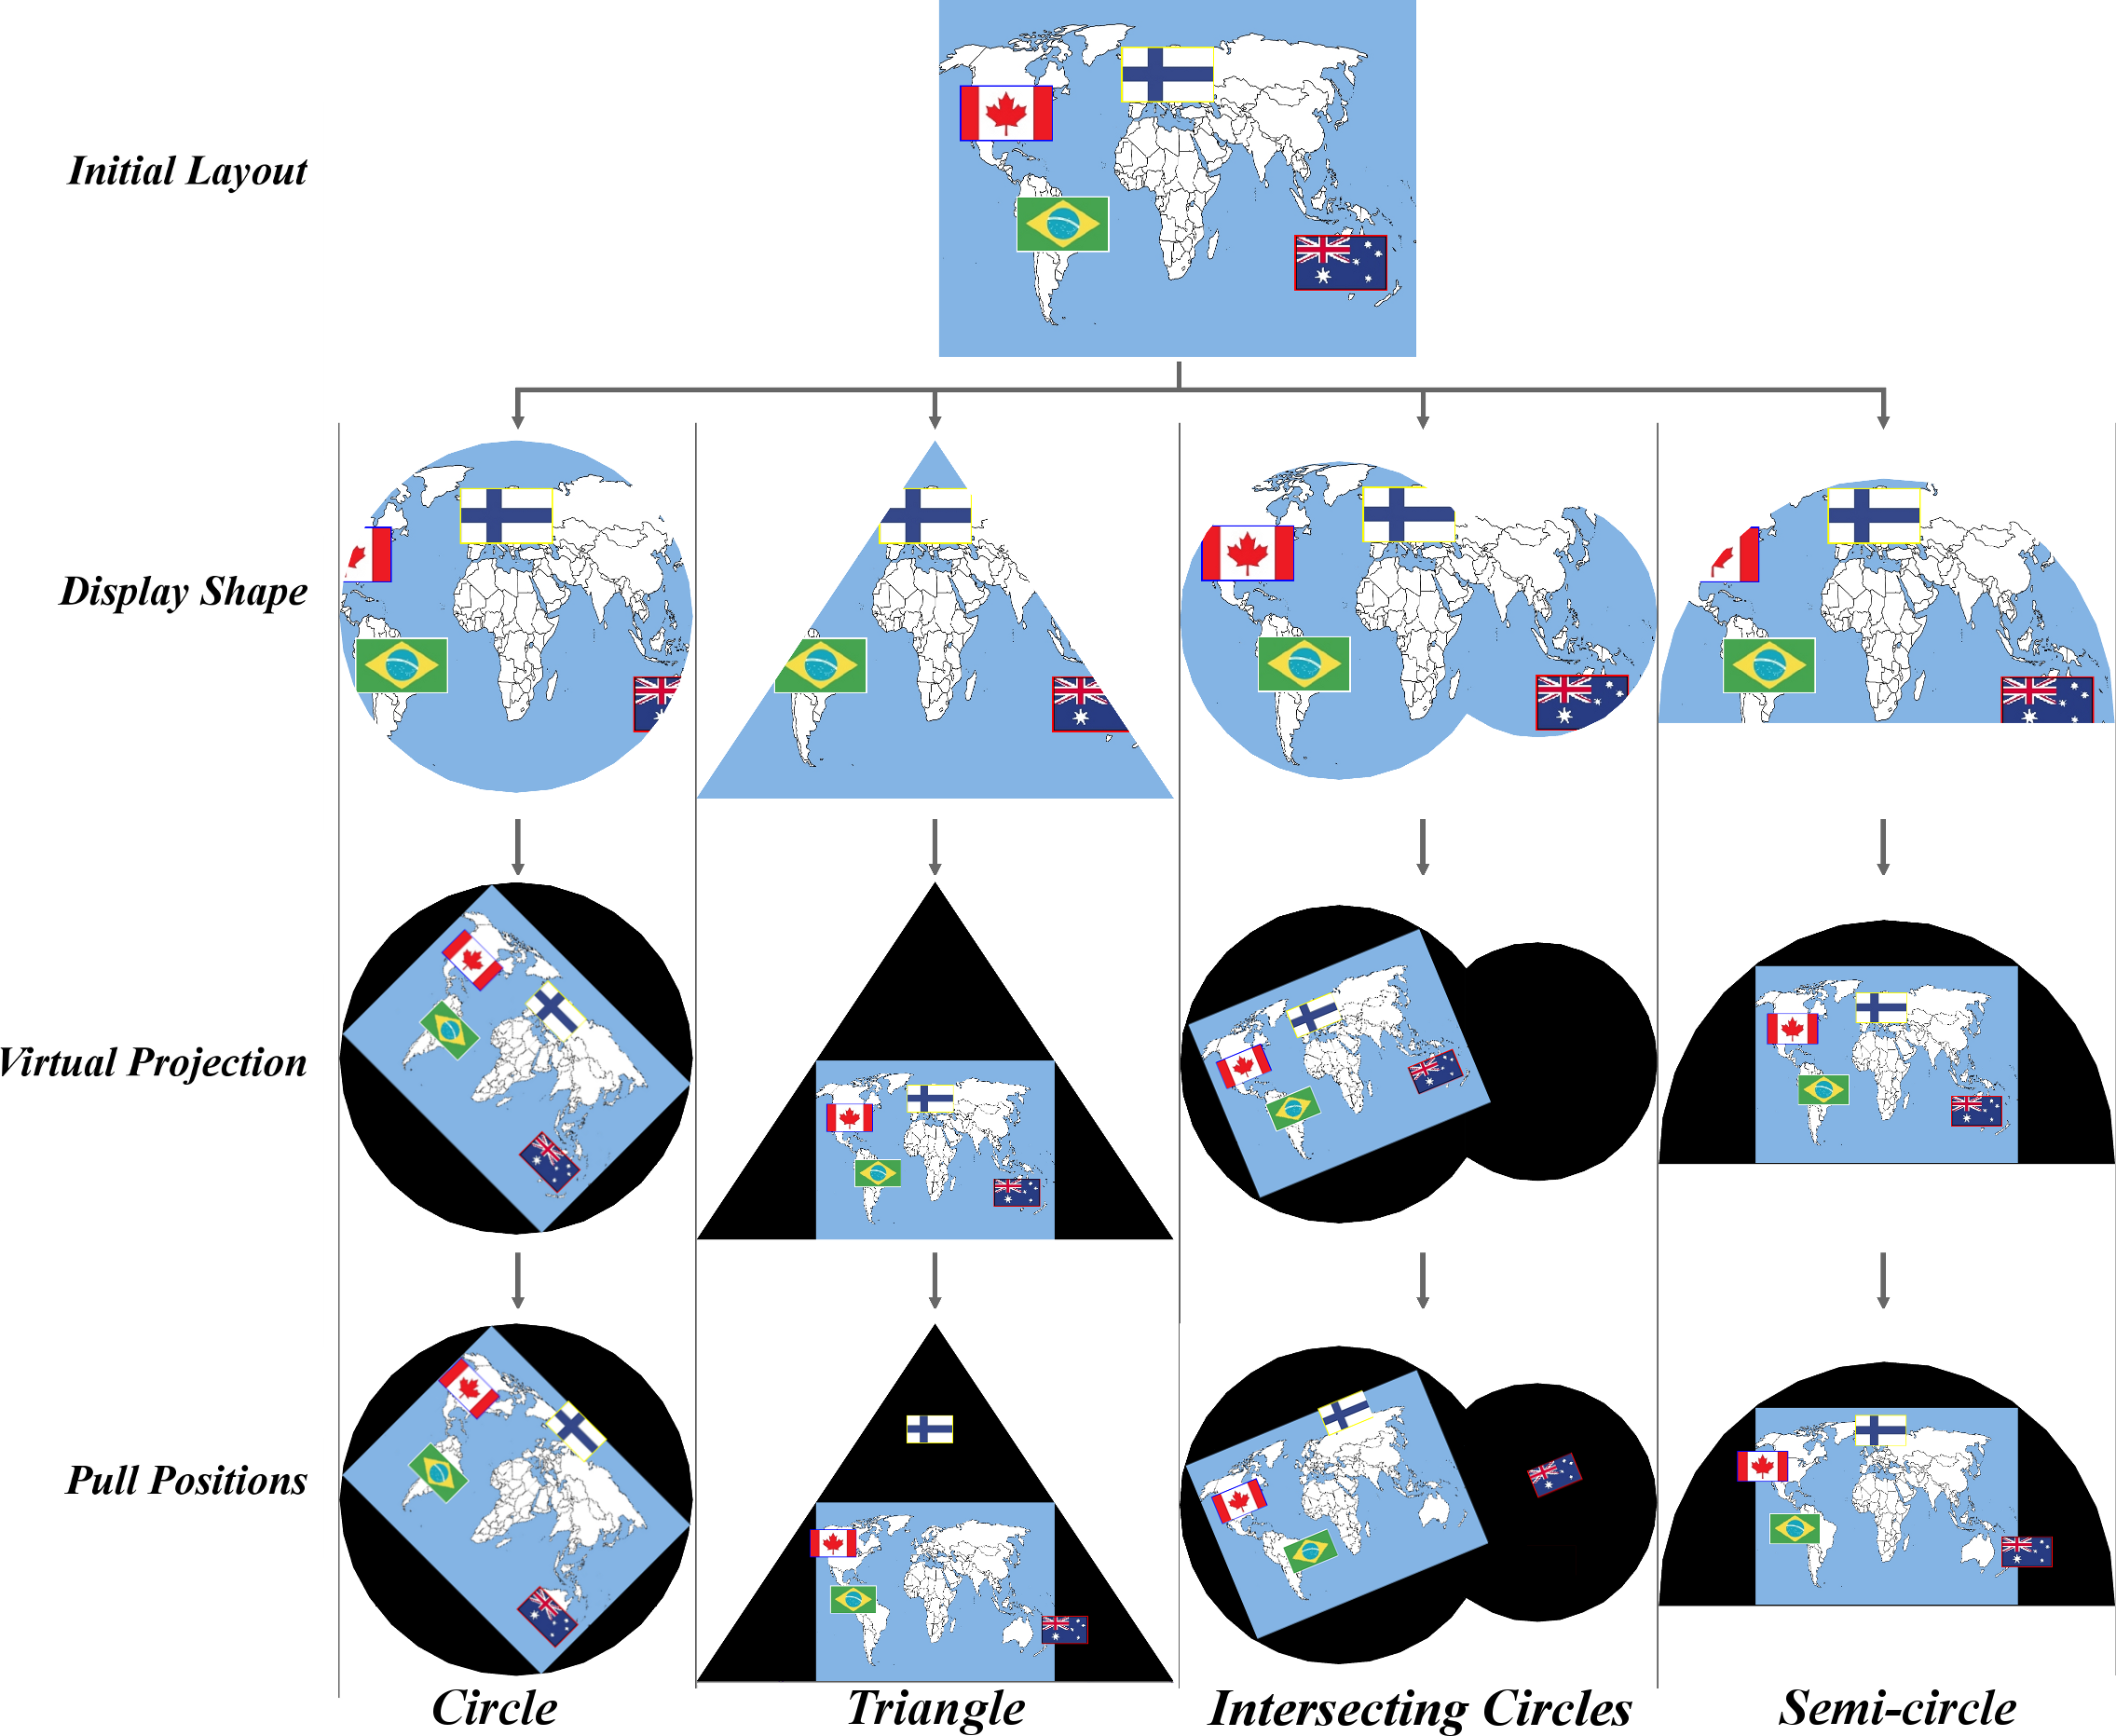
\includegraphics[width=1\textwidth]{figures/map_app.png}}
	\caption{Influence of the implemented technique on SynergyNet's Simple Map application.}
	\label{fig:mapApp}
\end{figure*}

Figure~\ref{fig:mapApp} shows the Simple Map application which consists of an item displaying a map which fills the background of the software environment.
On top of the map flags or images relating to specific countries are generated.
The application positions these items to appear on top of their respective countries.

It was observed during the study that developers may wish for some content items to be affected by it in different ways.
For example, a content item may be intended to act as a background to an application.
If the implemented \ac{DSDI}-minimising technique a system uses to adapt to different display shapes is unaware of this, the item would be scaled with the virtual projection.
This would have the effect of the background being constrained to a single region of the display, leaving other areas of the interface blank without a background.
In the implemented system, a method of making content item exempt from the influence of specific stages of the technique was made available.

In Figure~\ref{fig:mapApp} the map was made exempt from the influence of the position pulling stage of the technique.
If the map item was made exempt from both stages of the technique, the map would remain in the same position for all display shapes.
Though this would guarantee that the map would remain a background to the entire display, areas of it would be occluded which may not be desirable.
Therefore the map item was made to adhere to the virtual projection stage of the technique, but not the position pulling stage.
As a result of this, the map effectively represents the virtual projection on each display shape.
The placement of the virtual projection on the circle and intersecting circles display highlights how the contents may be rotated to fit the display shape.
Since the software is intended for use on a tabletop display this is not an issue.
This is because the horizontal nature of the display signifies that there is no single vantage point that the interface will be viewed from.

\begin{figure*}[t] 
 \centering
   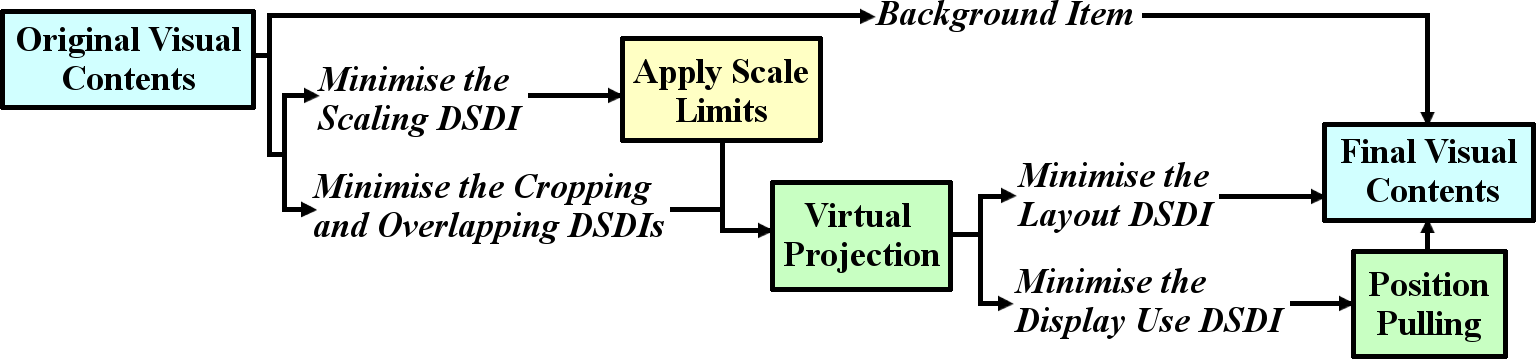
\includegraphics[width=1\textwidth]{figures/solution_flow.png}
   \caption{Flowchart demonstrating navigation of the technique.}
   \label{fig:flowchart}
\end{figure*}

Figure~\ref{fig:mapApp} demonstrates the importance of the layout of content items.
Up to the virtual projection stage of the technique the flag items correctly align with the countries on the map.
However, the position pulling stage deforms the layout of the flags in such a way that disengages this alignment.
If it is important for this alignment to be kept then it is best if the flags are made exempt from the position pulling stage of the technique.
As a consequence of this however, areas of the display will be left unused by the layout.
It therefore becomes a choice developers must make between whether to preserve the layout of content items or to maximise the usage of the display's real estate.
A clear example of this choice can be seen in the technique's influence on the Intersecting Circles display shape in Figure~\ref{fig:mapApp}.
Without the influence of the position pulling stage of the technique, a large region of the display is left unused by the initial layout.
This results in the Display Use \ac{DSDI} occurring.
However, with the influence of the position pulling stage of the technique, several of the flag items appear off the map, away from their respective positions, indicating the Layout \ac{DSDI} has occurred.

From the use of the implemented technique it was noted that in some scenarios the limits imposed on the scaling of content items by the technique could cause the Overlapping \ac{DSDI} to occur.
If content items positioned close to each other are scaled to their predetermined limits but the virtual projection, and therefore their layout, is scaled beyond this then occlusion may occur.
This occlusion is caused by the content items overlapping.
A potential adaptation of the virtual projection stage of the technique could resolve this.  
This adaptation makes use of the smallest box possible which encloses the content items, rather than using the shape of the entire original environment.
Any unused regions of the original display between the content items and the display's edges are ignored.
This variation of the technique could be used with any software where the distance between content items and the display edges does not need to be preserved.
By discarding the unused regions of the original display surrounding the content items, the virtual projection is likely to be smaller.
Therefore, the scaling required to fit the virtual projection into a new display shape will be reduced.
This diminishes the likelihood of content items and their layout being scaled to beyond their limits. 

Figure~\ref{fig:flowchart} shows the options available to developers utilising the technique.
Choices made in its implementation, such as which stages of the technique are employed and the constraints placed on these stages, can influence which \acp{DSDI} it prevents and counters.
For example, if a developer wishes a content item to act as the background to the entire display, and its cropping is not an issue, then both stages of the technique can be circumvented.
For content items not set aside to be background images developers can choose whether or not to apply the position pulling stage of the technique.
If applied the content items will maximise the use of the display shape's real estate by being pulled into previously unused areas of the display.
However, if the layout of the content items is of a greater importance than the maximisation of display usage, the developer can choose to disregard the position pulling stage for any content items in the layout.

In the SynergyNet implementation both stages of the technique are, by default, applied to content items whenever they are transformed using absolute values.
However, application developers using the framework have the option to override this for specific content items.
Application developers can apply changes to the technique, such as applying scale limits to the virtual projection, to all content in an application or to individual items.
The ability to choose which stages of the technique affect a content item gives developers control over it's influence.
Without this ability there is still a danger of intolerable \acp{DSDI} occurring in software despite the presence of the implemented technique.
This highlights the importance of any technique intended to minimise the influence of the potential \acp{DSDI} in a system not only to be capable of adapting to different display shapes, but to be also capable of adapting to the needs of the developer.

%-------------------------------------------------------------------------
\section{Conclusions and Future Work}
\label{sec:conclusion}

The development of the technique discussed in Section~\ref{sec:solution} has shown that when designing software for use on differently shaped tabletop displays, the Cropping \ac{DSDI} must be considered.
In addition to this, secondary \acp{DSDI} which can result from attempts to resolve the initial cropping must also be accounted for.
Developers should also consider which \acp{DSDI} their software can tolerate and which must be handled by a \ac{DSDI}-minimising technique.
Choices must be made between whether to preserve the layout of content items or to maximise the display usage.

Developers must consider the implementation of any proposed method of countering the \acp{DSDI}.
The identification, or creation of, an adequate \ac{DSDI}-minimising technique which allows a particular system to adapt to different display shapes could form part of design guidelines for emerging technologies.
It is important to note that not only the list of \acp{DSDI} for a system should influence the design of a \ac{DSDI}-minimising technique.
The need for applications to control the magnitude of a \ac{DSDI}-minimising technique's influence is important to consider.

\begin{figure}[h]
 \centering
   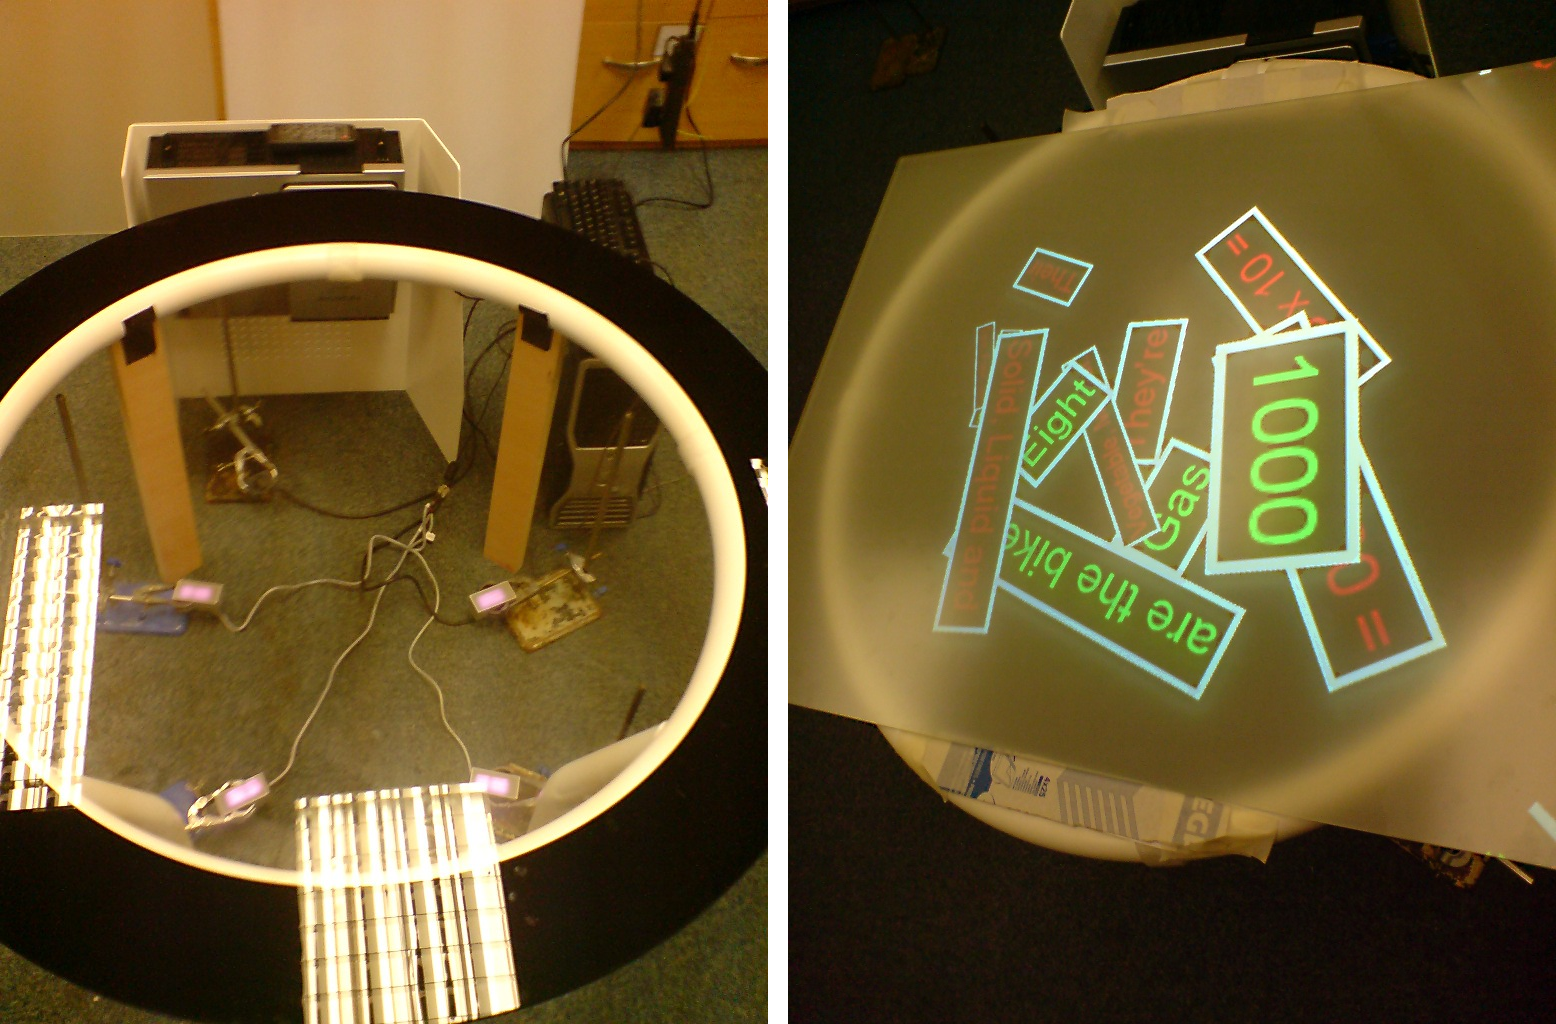
\includegraphics[width=0.45\textwidth]{figures/prototype.png}
   \caption{A prototype of a circular tabletop display.}
   \label{fig:prototypeTabletop}
\end{figure}

There are a number of reasons why it is important that software becomes display shape independent.
There is now a growing drive for software to become ubiquitous with the increased availability of natural user interfaces.
For a system to become ubiquitous it must fit its environment~\cite{Greenfield2006}.
Being able to change the display shape of a system would aid in achieving this.

% TODO More here on need for this work

Figure~\ref{fig:prototypeTabletop} shows a prototype built of a circular tabletop interface intended for use as an interactive kiosk for public spaces.
The lack of readily available software for the interface's circular display meant that if the tabletop was to be used then bespoke software would need to be commissioned at a cost to the manufacturer rather than using any of the readily available off-the-shelf products intended for interactive kiosks.

% TODO Highlight lack of innovation in this area in recent years.


With a system capable of utilising different display shapes, research into the effect of a display shape on the use of the system can be carried out.
Prototyping can be employed to investigate how the shape of a display influences the interaction between users and the system.
Some shapes may be found better suited to certain users or tasks.
With this knowledge the design of future systems could utilise display shapes suited to their audiences or purposes.

The technique outlined in Section~\ref{sec:solution} could be used beyond tabletop systems.
However, it is possible for the \acp{DSDI} in other systems to vary. 
For example, attempts to resolve the initial Cropping \ac{DSDI} may require content items to be rotated.
If a user is viewing the display from a single perspective, such as with a vertical display, then any change in content item's orientation is undesirable.
Information displayed by visual content items, such as text, could appear upside down to the user, making it difficult to comprehend.
However, it is not an issue for systems which allow users to view from multiple perspectives around the display, such as those which utilise horizontal interfaces.
Future work could entail the outlining of \ac{DSDI} for other sets of systems and the production of techniques to minimise their influences.

The technique produced in this paper can be used in several scenarios.
One such use of the technique is its implementation into the application layer of a piece of software.
This would allow a specific layout of visual content items to be dynamically adapted to different display shapes.
As this implementation of the technique would be customised to the application's specific layout, it would ensure the best results.
However, this does have the drawback that the technique would need to be redefined for every unique application.

Another use for the technique is its implementation into a framework.
In a framework level implementation, the same technique can be employed by various applications to adapt their visual contents to different display shapes.
This is similar to how systems like SUPPLE~\cite{Gajos2004} adapt contents to display parameters.
However, a drawback to this approach is that the technique's implementation may not be suitable for some applications.  
For example, if the technique implementation does not enforce scale limits the Scaling \ac{DSDI} may occur.
This may be acceptable for some applications, such as those intended to use content which can still communicate information to the user at any size.
However, it would be intolerable for other applications, such as those using text.
Therefore, it is important when implementing this technique at a framework level that applications can change how the technique influences them.
The technique's use of higher level functions, such as the ray firing used in the position pulling stage, make it unsuitable for implementation in lower level software.

The technique could also be implemented as part of a design tool which is used to adapt the layout of visual contents, similar to GUMMY~\cite{Meskens2008}.
Using this implementation, software developers can use the resulting tool to adapt a layout of content items to a specific display shape.
Developers can then make any further changes manually if the tool's automatically generated \ac{DSDI}-minimising technique is not adequate.
Once a developer is satisfied with the software layout they can then specify for its use in their software when the appropriate display shape is present.
This approach has the advantage of allowing developers to check that the layout will be suitable for a specific shape.
However, it does limit the display shapes the system can use to those the developer has input into the tool.

The technique could be transformed into a set of guidelines for developers to follow when creating software interfaces without the use of a design tool.
The guidelines could also incorporate the decisions to be made concerning the trade-offs in which \acp{DSDI} are minimised.
These guidelines could then be formalised~\cite{Ngo2000} allowing their application to software to be automated in places.
This would aid with the technique integrations into with frameworks and design tools.
With the technique implemented in a tool used to design a wider range of software its influence can be tested on a wider range of user interfaces with varying complexities in future studies.

The technique produced in this paper is capable of minimising the effect of the identified \acp{DSDI} but requires trade-offs.
Developers using the technique must decide which \acp{DSDI} could not be tolerated by their software and must adapt the technique according.
Future tabletop software development would benefit greatly from the creation of guidelines to be followed when adapting software to become display shape independent.
The technique produced in this paper, or another similar \ac{DSDI}-minimising technique, could form part of these guidelines.

%-------------------------------------------------------------------------
\section*{Acknowledgements}

This work was partially funded by the EPSRC ERSC TLRP SynergyNet project (Grant RES-139-25-0400).

%-------------------------------------------------------------------------

\bibliographystyle{elsarticle-num}
\bibliography{DifferentDisplayShapesReferences}


%-------------------------------------------------------------------------

\end{document}